\documentclass{beamer}

\usepackage[
backend=biber, 
style=apa]{biblatex}

\usetheme{metropolis}  
%\renewcommand*{\bibfont}{\normalfont\tiny}

\title{Power failure: Why small sample size undermines the reliability of neuroscience}
\subtitle{Katherine S. Button, John P. A. Ioannidis, Claire Mokrysz, Brian A. Nosek, Jonathan Flint, Emma S. J. Robinson and Marcus R. Munafò \\~\\ NATURE REVIEWS | NEUROSCIENCE VOLUME 14 | MAY 2013}
\date{\today}
\author{Quentin Lam}
%\institute{Department of Psychology, the Chinese University of Hong Kong}
\titlegraphic{
    \flushright
\includegraphics[height=1cm]{CUHK/CUHK_name.pdf}
}
\addbibresource{presentations.bib}

\begin{document}
    \maketitle
    
    \begin{frame}
    	\begin{figure}[H]
    		\centering
    		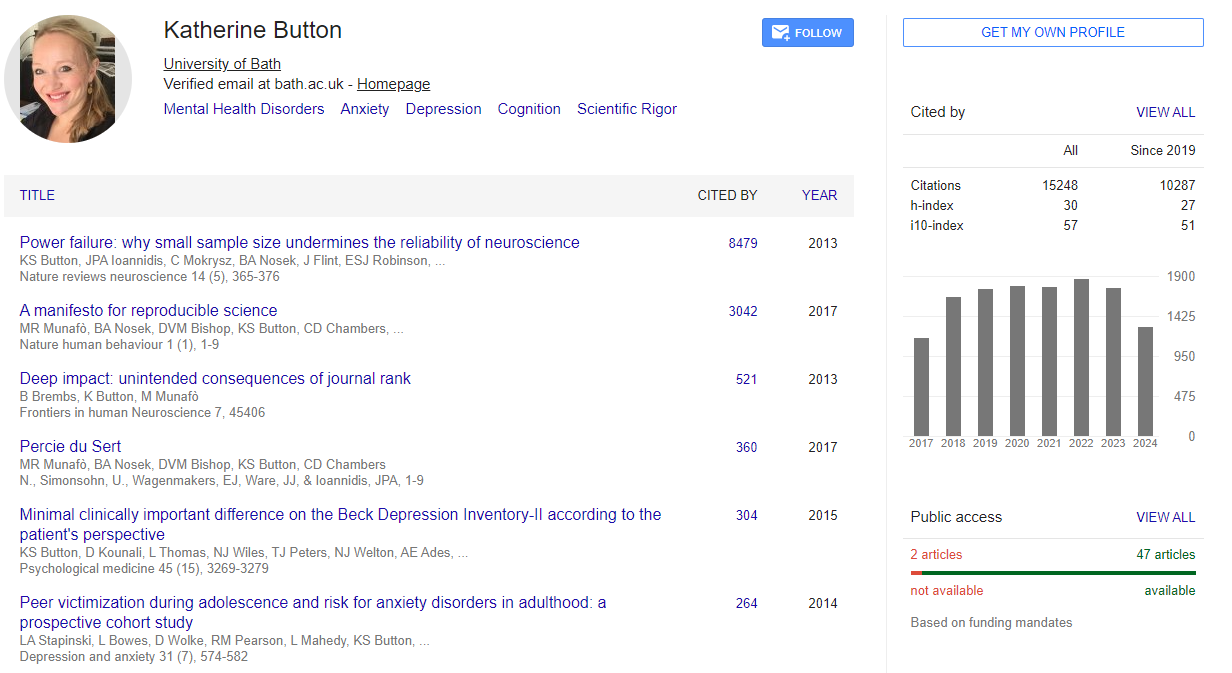
\includegraphics[width=1\textwidth]{pics/first author.png}
    	\end{figure}
    \end{frame}
    
    \begin{frame}
    	\begin{figure}[H]
    		\centering
    		
\includegraphics[width=1\textwidth]{pics/corrspondence author.png}
    	\end{figure}
    \end{frame}
    
    \tableofcontents

    \section{Introduction: What makes studies unreproducible}
    \begin{frame}{Reproducibility crisis in psychology}
    	\begin{figure}[H]
    		\centering
    		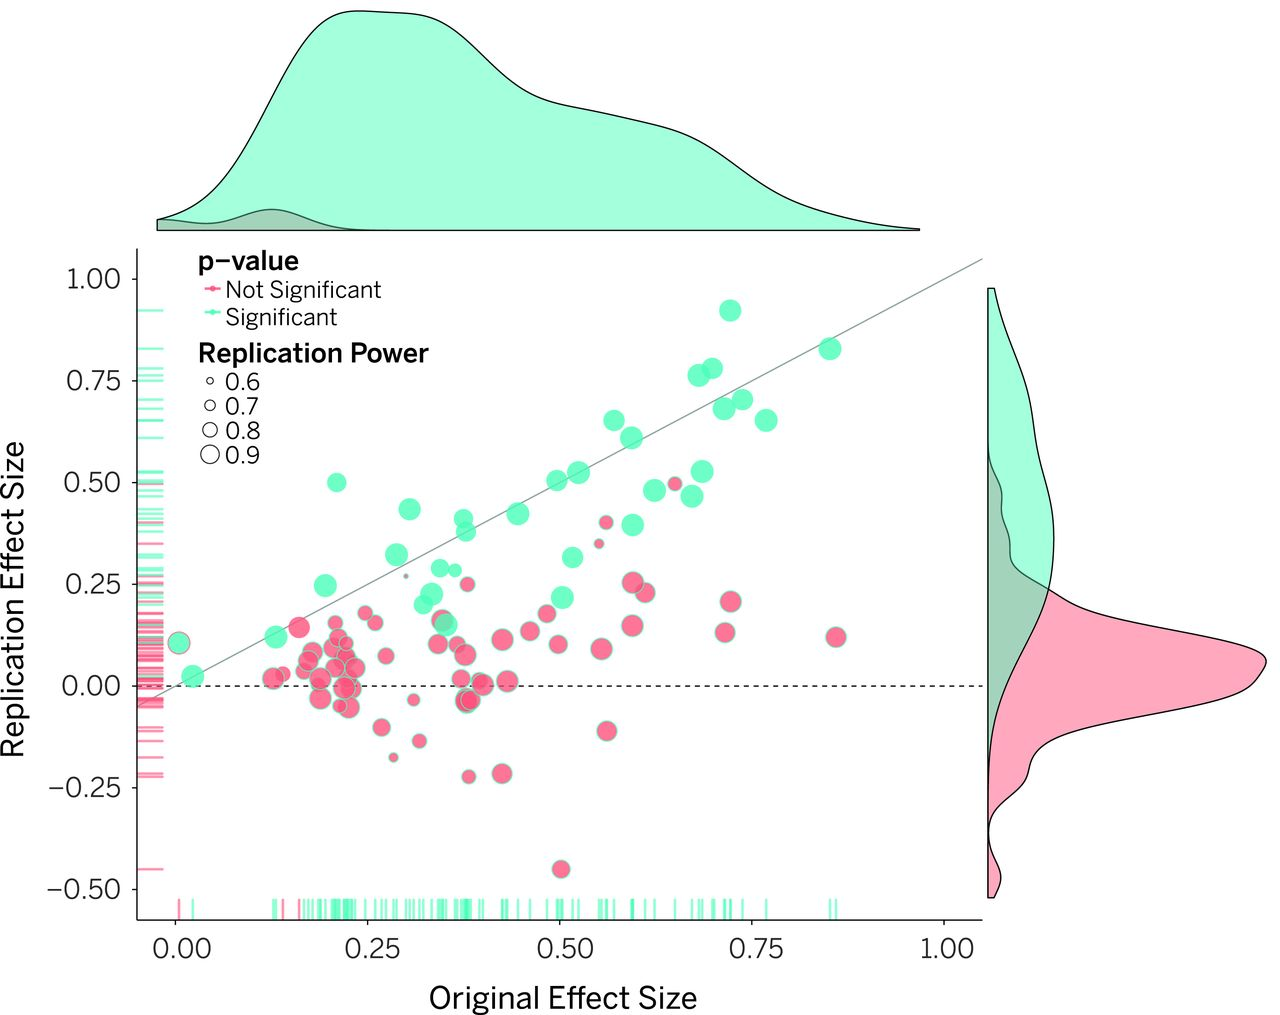
\includegraphics[width=.8\textwidth]{pics/effect size.jpeg}
    		\caption{Original study effect size versus replication effect size (correlation coefficients) (\cite{opensciencecollaboration2015}).}
%    		\label{fig:figure1}
    	\end{figure}
    \end{frame}

    \begin{frame}{Statistical trap}
    	\begin{columns}
          \column{.5\textwidth}
    	\begin{itemize}
   		  \item Flexible experiment design
          \item Flexible statistical analyses
          \item Small sample size
      	\end{itemize}
			\column{.1\textwidth}
			$\Longrightarrow$
            \column{.5\textwidth}
            \begin{itemize}
            	\item Lower statistical power
            	\item Higher false positive rate
            \end{itemize}
        \end{columns}
        
       ~\\In bio medicine, 97\% genetic association studies have at least one false positive results (\cite{sullivan2007}). 
    \end{frame}
    
    \begin{frame}{Intuition of power}
%    	A study attempting to replicate a nominally significant effect (p ~ 0.05), which uses the same sample size as the original study, would therefore have (on average) a 50\% chance of rejecting the null hypothesis (indicated by the coloured area under the green curve) and thus only 50\% statistical power.
    	\begin{figure}[H]
    		\centering
    		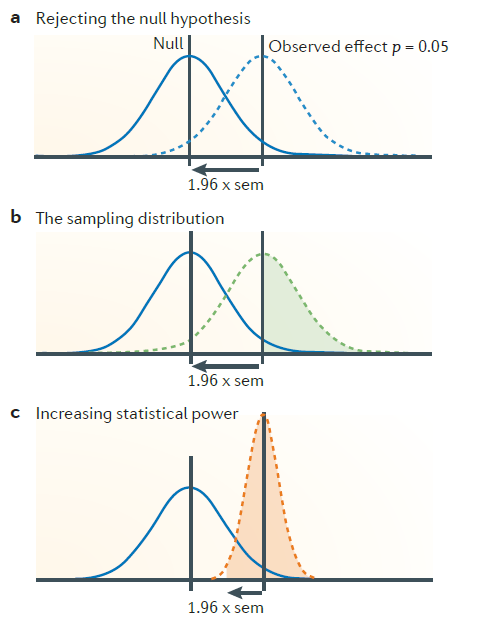
\includegraphics[width=0.59\textwidth]{pics/power intuitive graph.png}
    	\end{figure}
    \end{frame}
    
    \begin{frame}{Power definition}
    	\fontsize{10pt}{12pt}\selectfont
    	The statistical power of a study is the probability of correctly rejecting the null hypothesis and detecting a statistically significant result (not committing a type II error) (\cite{wheeler2014}).
    	\begin{figure}[H]
    		\centering
    		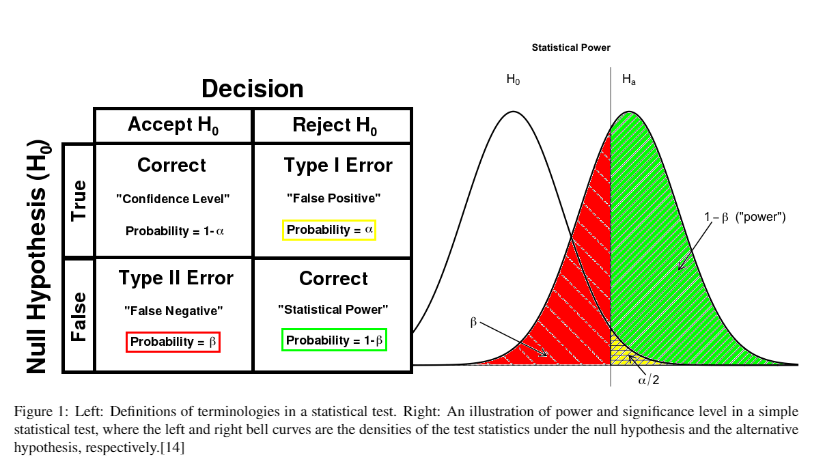
\includegraphics[width=1\textwidth]{pics/power.png}
    	\end{figure}
    \end{frame}
    
    \begin{frame}{Power examination}
    \href{https://rpsychologist.com/d3/nhst/}{https://rpsychologist.com/d3/nhst/}
    
    \begin{figure}[H]
    	\centering
    	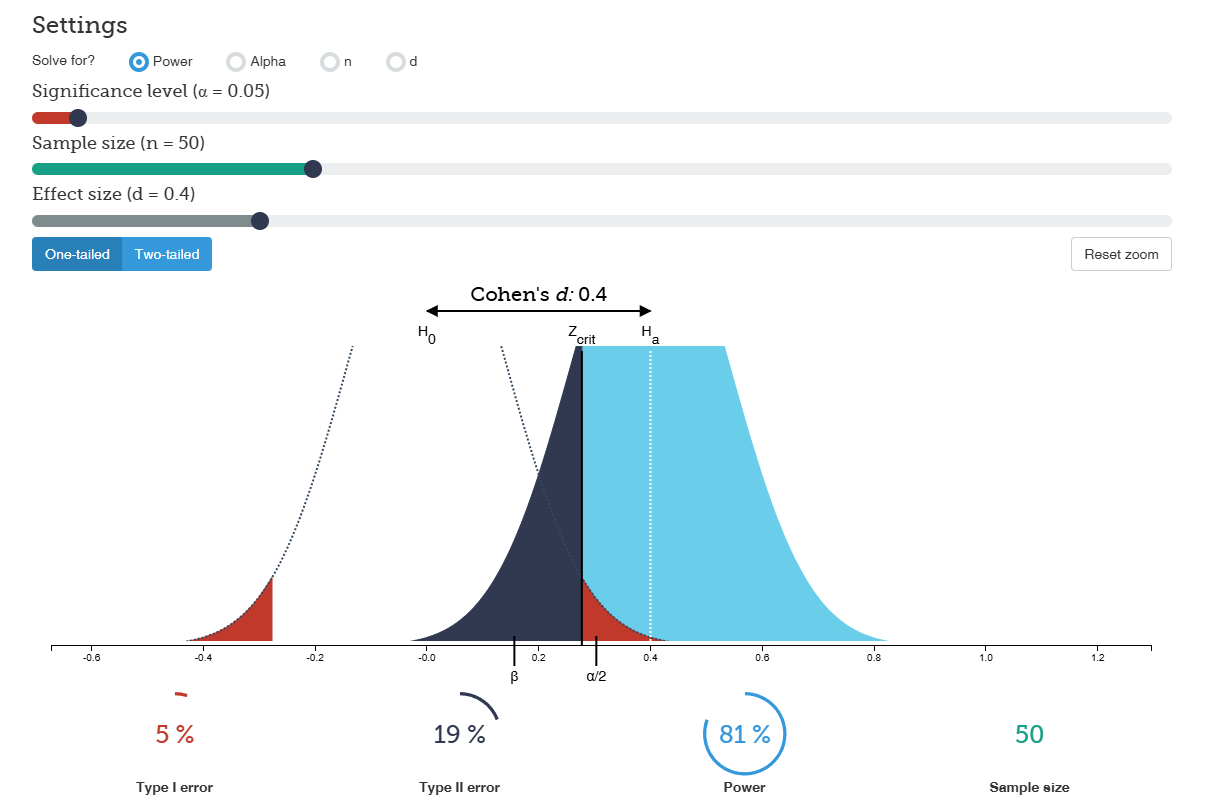
\includegraphics[width=1\textwidth]{pics/power demo.png}
    \end{figure}
	\end{frame}
	
    \section{How low power affects study reliability without other biases}
	
	\begin{frame}{Low power without other biases}
		3 problems in low power studies:
		\begin{itemize}
			\item Low probability of finding true effects 
			\item Low positive predictive value when an effect is claimed
			\item Exaggerated estimate of the effect magnitude when a true effect is discovered
		\end{itemize}
	\end{frame}
	
	\begin{frame}{P 1/3: Low probability of finding true effects}
		Low power means that the chance of discovering effects that are genuinely true is low.
		
		\fontsize{10pt}{12pt}\selectfont
		E.g., When studies in a given field are designed with a power of 20\%, it means that if there are 100 genuine non-null effects to be discovered in that field, these studies are expected to discover only 20 of them.
		
		\begin{figure}[H]
			\centering
			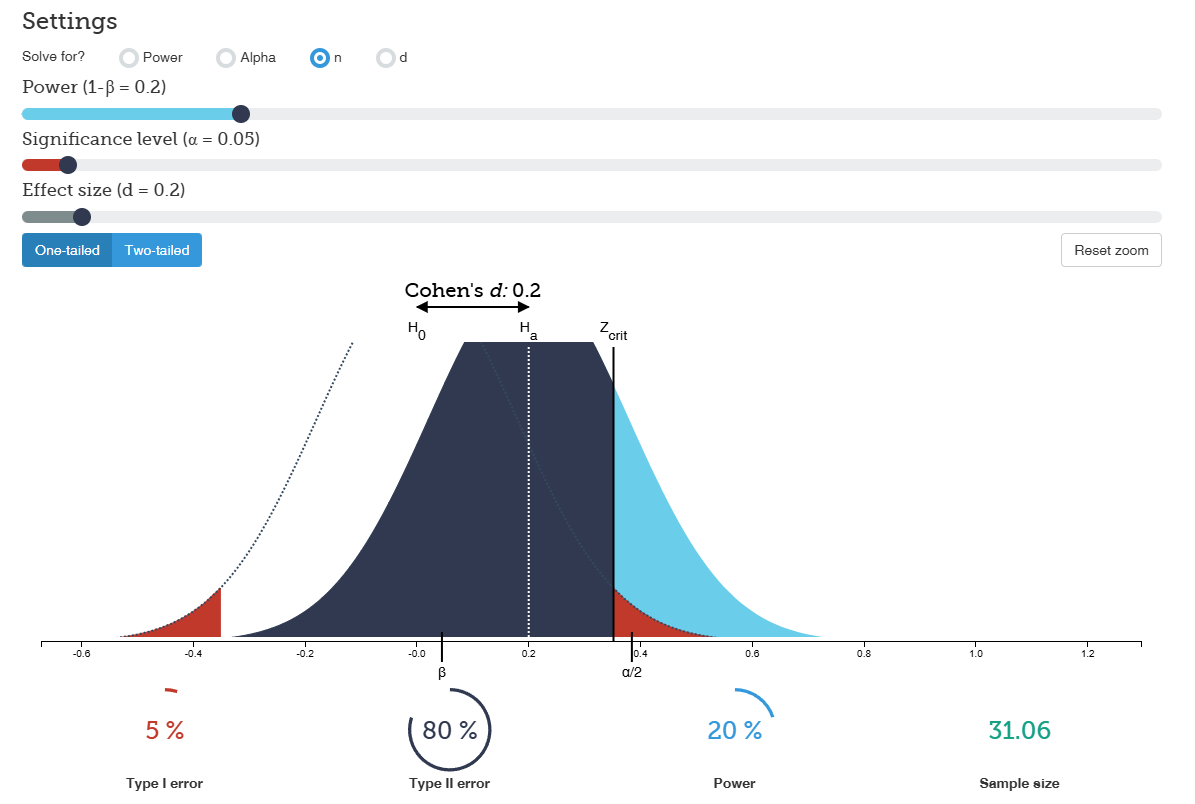
\includegraphics[width=0.7\textwidth]{pics/low power demo.png}
		\end{figure}
	\end{frame}
	
	\begin{frame}{P 2/3: Low positive predictive value when an effect is claimed}
		The lower the power of a study, the lower the probability that an observed effect that passes the required threshold of claiming its discovery (that is, reaching nominal statistical significance, such as p< 0.05) actually reflects a true effect. 
		
		~\\ \fontsize{9pt}{11pt}\selectfont
		\begin{align*}
		\mathrm{Positive Predictive Value (PPV) = \frac{([1 - \beta] \times R)}{([1 - \beta] \times R + \alpha)}}
		\end{align*}
		\begin{center}
			$\Downarrow$
		\end{center}
		\fontsize{9pt}{11pt}\selectfont
		\[\mathrm{Positive Predictive Value (PPV) = \frac{(Power \times Prestudy Odds)}{(Power \times Prestudy Odds + Type  \uppercase\expandafter{\romannumeral1} Error Rate)}}\]
		
		~\\ \textbf{R} is the pre-study odds (that is, the odds that a probed effect is indeed non-null among the effects being probed).
	\end{frame}
	
	\begin{frame}{P 2/3: Low positive predictive value when an effect is claimed}
		~\\ \fontsize{9pt}{11pt}\selectfont
		\[\mathrm{Positive Predictive Value (PPV) = \frac{(Power \times Prestudy Odds)}{(Power \times Prestudy Odds + Type  \uppercase\expandafter{\romannumeral1} Error Rate)}}\]
		
		Power $\uparrow$, PPV $\uparrow$. Type $\uppercase\expandafter{\romannumeral1}$ error rate $\uparrow$, PPV $\downarrow$.
		
		E.g., if $\frac{1}{5}$ effects we test are expected to be truly non-null (that is, $R = \frac{P(Discover Effect)}{P(Discover No Effect)} = \frac{1}{5 - 1} = 0.25$), 
		
		and the discovered effect $p < .05$, if have 20\% power, then 
		
		$PPV = \frac{0.20 \times 0.25}{0.20 \times 0.25 + 0.05} = \frac{0.05}{0.10} = 0.50$ 
		
		that is, only half of the findings would be correct.
		
		if power = 0.8, then 
		
		$PPV = \frac{0.80 \times 0.25}{0.80 \times 0.25 + 0.05} = \frac{0.20}{0.25} = 0.80$  
		
		which means 80\% of our findings would be correct. 
	\end{frame}
	
	\begin{frame}{P 3/3: Exaggerated estimate of the effect magnitude when a true effect is discovered}
		\fontsize{10pt}{12pt}\selectfont
		Winner's curse: Lower power exaggerate the effect magnitude, especially based on the statistical significance(i.e., $p$ value, BF value)
		
		\fontsize{10pt}{12pt}\selectfont
		E.g., Medium True effect size, small studies can only pass the discovery threshold by overestimating the effect magnitude.
		
		\begin{columns}
			\column{.6\textwidth}
			\begin{figure}[H]
				\centering
				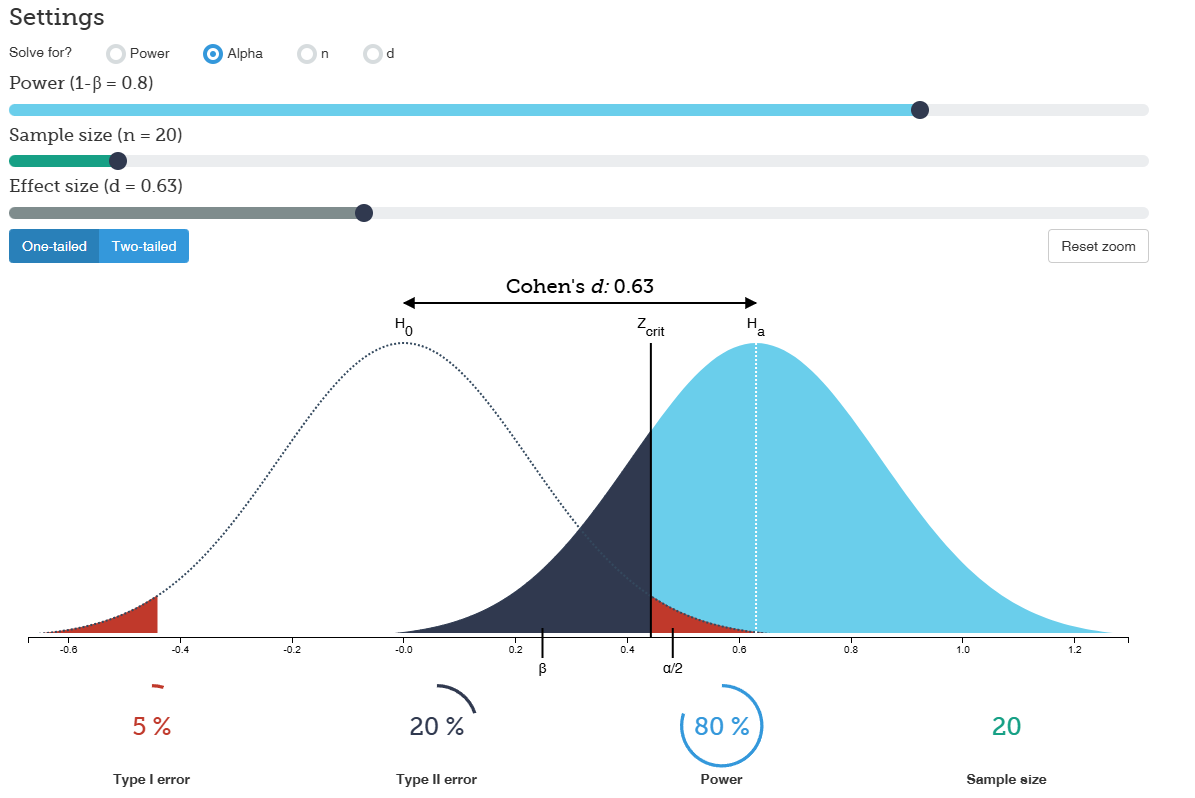
\includegraphics[width=0.7\textwidth]{pics/effect size small sample.png}
			\end{figure}
			\column{.6\textwidth}
			\begin{figure}[H]
				\centering
				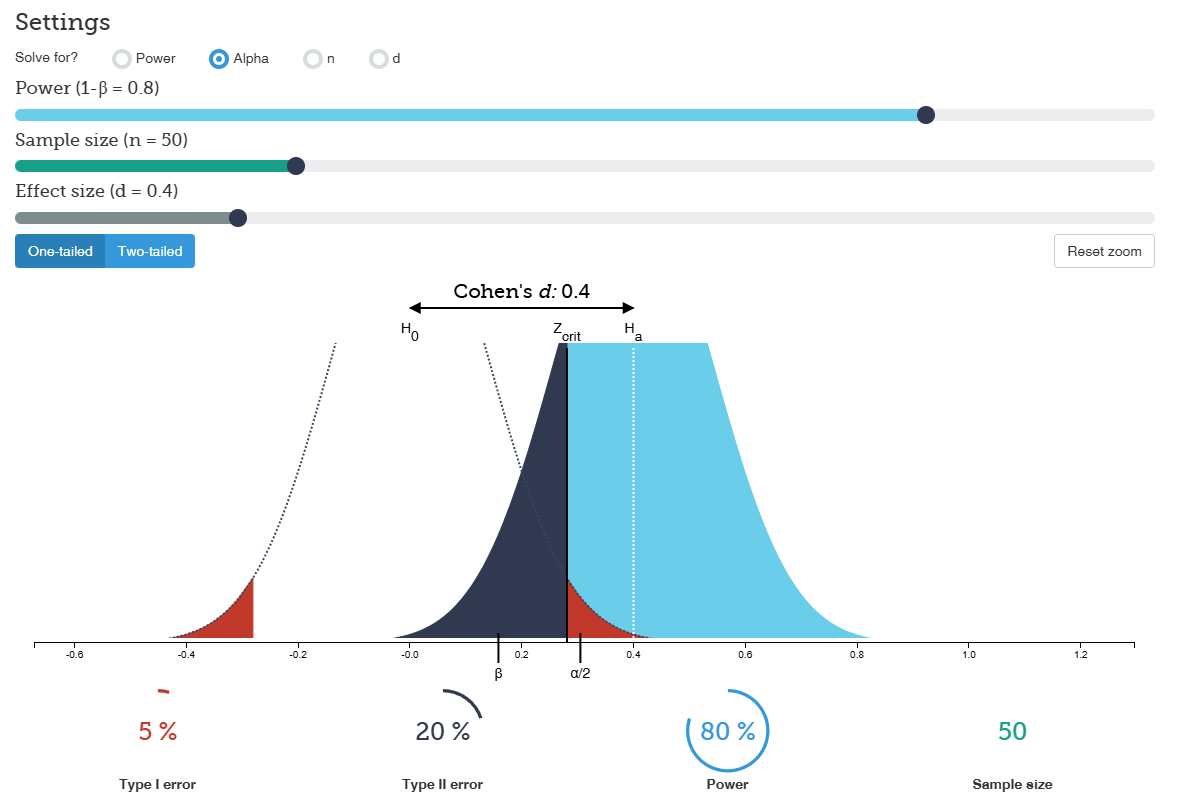
\includegraphics[width=0.7\textwidth]{pics/effect size large sample.png}
			\end{figure}
		\end{columns}	
	\end{frame}
	
	\begin{frame}{P 3/3: Exaggerated estimate of the effect magnitude when a true effect is discovered}
		To illustrate the winner’s curse, suppose that true effect R(Pre-study odds) =  1.20.
		
		\fontsize{10pt}{12pt}\selectfont
		Our study only has power that is 20\% to detect an odds ratio of 1.20.
		
		\fontsize{10pt}{12pt}\selectfont
		\begin{itemize}
			\item Sampling variation
			\item Random error in the measurements
		\end{itemize}
		
		\fontsize{10pt}{12pt}\selectfont
		Because of random errors, our study may in fact find an odds ratio fluctuate around 1.20 (e.g., 1.00 or 1.60). Odds ratios of 1.00 or 1.20 will not reach statistical significance because of the small sample size. Only when the odds ratio is 1.60 can claim significance. 
		
		\fontsize{10pt}{12pt}\selectfont
		The winner’s curse means that the ‘lucky’ scientist who makes the discovery in a small study is cursed by finding an inflated effect.
	\end{frame}
	
	\section{How low power affects study reliability \textbf{with other biases}}
	
	\begin{frame}{How low power affects study reliability with other biases}
		3 problems in low power studies:
		\begin{itemize}
			\item Vibration of effects
			\item Publication bias
			\item Low quality design
		\end{itemize}
	\end{frame}
	
	\begin{frame}{P 1/3: Vibration of effects}
		Vibration of effects: Study obtains different estimates of the effect magnitude depending on the analytical options it implements.
		
		\begin{itemize}
			\item Statistical model
			\item Definition of the variables of interest
			\item Use (or not) of adjustments for certain potential confounders but not others
			\item Filters to include or exclude specific observations
			~\\ ......
		\end{itemize}
		
		\fontsize{10pt}{12pt}\selectfont
		In small studies, the range of results that can be obtained owing to vibration of effects is wider than in larger studies, because the results are more uncertain and therefore fluctuate more in response to analytical changes.
	\end{frame}
	
	\begin{frame}{P 2/3: Publication bias and selective reporting}
		Investigations into publication bias often examine whether small studies yield different results than larger ones.
		
		~\\A ‘negative’ result in a high-powered study cannot be explained away as being due to low power. 
		
		~\\Thus reviewers and editors may be more willing to publish large studies, whereas they more easily reject a small ‘negative’ study as being inconclusive or uninformative.
		
		~\\The protocols of large studies are also more likely to be publicly available, so that deviations in the analysis plans and choice of outcomes may become obvious more easily.
	\end{frame}
	
	\begin{frame}{P 3/3: Low quality design}
		Large studies often require more funding and personnel resources, so the designs are examined more carefully before data collection, and analysis and reporting may be more structured.
		
		~\\A favour of small studies may occur if the small studies are meticulously designed and collect high-quality data (and therefore are forced to be small) and if large studies ignore or drop quality checks in an effort to include as large a sample as possible.
	\end{frame}
	
	\section{Method}
		
	\begin{frame}{Meta-analyses inclusion flow diagram}
		\begin{columns}
			\column{.7\textwidth}
			\begin{figure}[H]
				\centering
				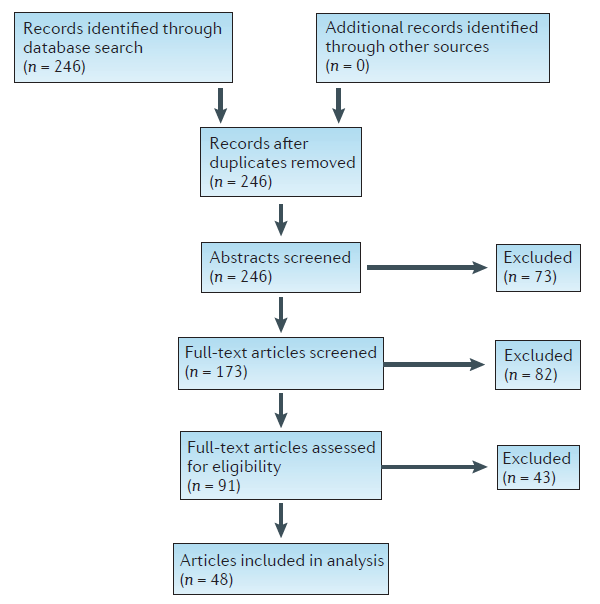
\includegraphics[width=0.7\textwidth]{pics/method.png}
			\end{figure}
			
			\column{.5\textwidth}
			\begin{itemize}
				\item Two authors (K.S.B. and M.R.M.) independently screened all papers
				\item Exclude no abstract
				\item Exclude no full-text
				\item Include 49 meta-analyses with 730 studies
				\item If meta-analyses have overlapped studies, include one with more studies overall
				\item If studies have missing data, then don't include it in the meta-analyses
				
			\end{itemize}
		\end{columns}
		
	\end{frame}
	
	\section{Results}
	
	\begin{frame}{Median power in Neuroscience}
		The median power is 21\%
		
		\fontsize{10pt}{12pt}\selectfont
		~\\Test for an excess of statistical significance: 349 out of 740 studies significant was higher than the number expected (254; $p < 0.0001$).
		
		\fontsize{10pt}{12pt}\selectfont
		~\\Almost 50\% of studies had an average power lower than 20\%, median statistical power in reliable sample size studies is 18\%
		
		
		\begin{figure}[H]
			\centering
			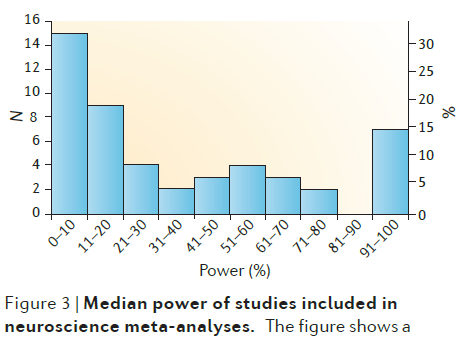
\includegraphics[width=0.6\textwidth]{pics/median power.png}
		\end{figure}
	\end{frame}
	
	\begin{frame}{Excess significance bias in Neuroimaging and animal studies}
		the fMRI studies median statistical power was 8\% across 461 individual studies contributing to 41 separate meta-analyses.
		
		\begin{figure}[H]
			\centering
			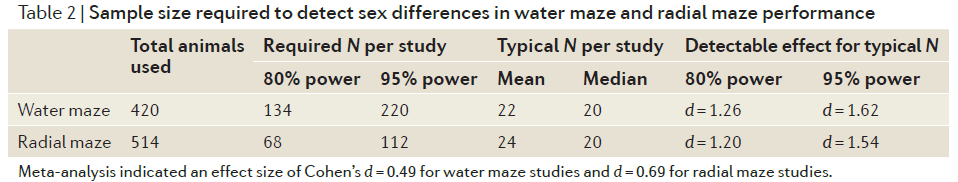
\includegraphics[width=1\textwidth]{pics/animal power.png}
		\end{figure}
	\end{frame}
	
	\section{Discussions}
	
	\begin{frame}{Implications for the likelihood that a research finding reflects a true effect}
		 The average statistical power of studies in the field of neuroscience is probably no more than between $\sim$8\% and $\sim$31\%,
			
		\begin{figure}[H]
			\centering
			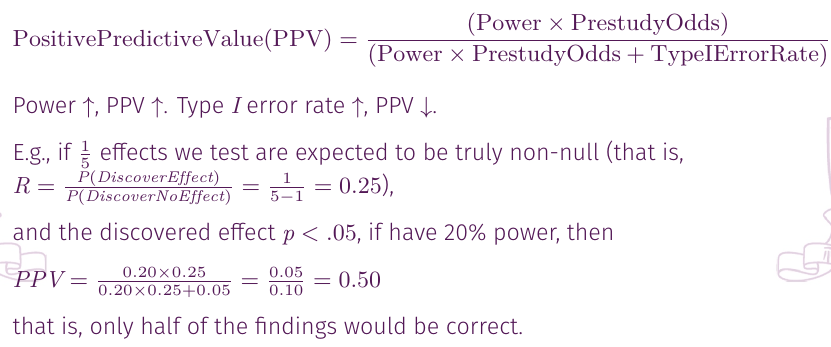
\includegraphics[width=1\textwidth]{pics/discussion likelihood.png}
		\end{figure}
	\end{frame}
		
	
	\begin{frame}{Positive predictive value as a function of the pre-study odds of association for different levels of statistical power}
		\begin{figure}[H]
			\centering
			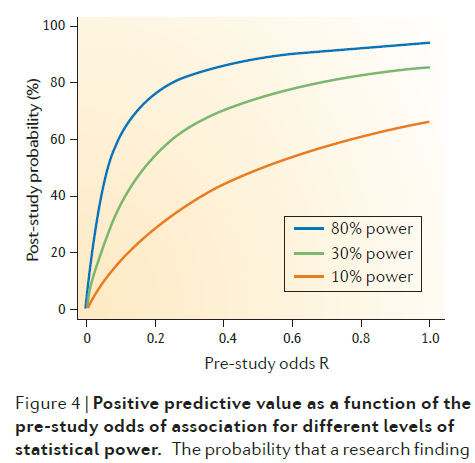
\includegraphics[width=0.87\textwidth]{pics/PPV discussion.png}
		\end{figure}
	\end{frame}
	
	\begin{frame}{The winner’s curse: Effect size inflation as a function of statistical power}
		\fontsize{10pt}{12pt}\selectfont
		These simulations suggest that initial effect estimates from studies powered between $\sim$8\% and $\sim$31\% are likely to be inflated by 25\% to 50\%. Inflated effect estimates make it difficult to determine an adequate sample size for replication studies, increasing the probability of type $\uppercase\expandafter{\romannumeral2}$ errors.
		\begin{figure}[H]
			\centering
			\includegraphics[width=0.5\textwidth]{pics/winner curse discussion.png}
		\end{figure}
	\end{frame}
	
	

	
	\begin{frame}{Real study power is even lower}
		Above simulation only consider R and power, did not consider several other biases that reduce the probability that a research finding reflects a true effect. 
		
		~\\Excess of significance test showed these studies effect sizes are inflated.
	\end{frame}
	
	\section{Conclusions and future directions}
	
%	\begin{frame}{Conclusions and future directions}
%		\begin{itemize}
%			\item{Increase disclosure}
%			
%			False positives occur more frequently and go unnoticed when degrees of freedom in data analysis and reporting are undisclosed.~\\
%			
%			\item{Registration of confirmatory analysis plan}
%			
%			Pre-registration and, ultimately, full reporting of analysis plans clarifies the distinction between confirmatory and exploratory analysis, encourages well-powered studies (at least in the case of confirmatory analyses) and reduces the file-drawer effect.~\\
%			
%			\item{Improving availability of materials and data}
%			
%			The Dataverse Network Project and Dryad for data in general and others such as OpenfMRI, INDI and OASIS for neuroimaging data in particular, most recommended OSF.
%			\item{Incentivizing replication}
%			
%			For example, journals could offer a submission option for registered replications of important research results (see, for example, a possible new submission format for Cortex (see \cite{chambers2013})~\\
%			
%		\end{itemize}
%	\end{frame}
	
	\begin{frame}{Conclusions and future directions}		
		\begin{figure}[H]
			\centering
			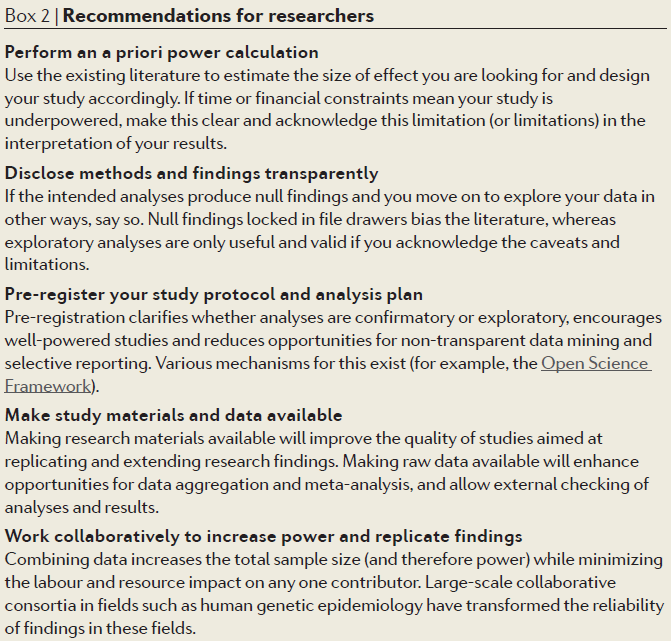
\includegraphics[width=0.7\textwidth]{pics/recommend for researcher.png}
		\end{figure}
	\end{frame}
	
	\section{Take home messages} 
		
	\begin{frame}{Sample size should at least double for replication study}	
		\begin{columns}
			\column{.6\textwidth}
			\begin{figure}[H]
				\centering
				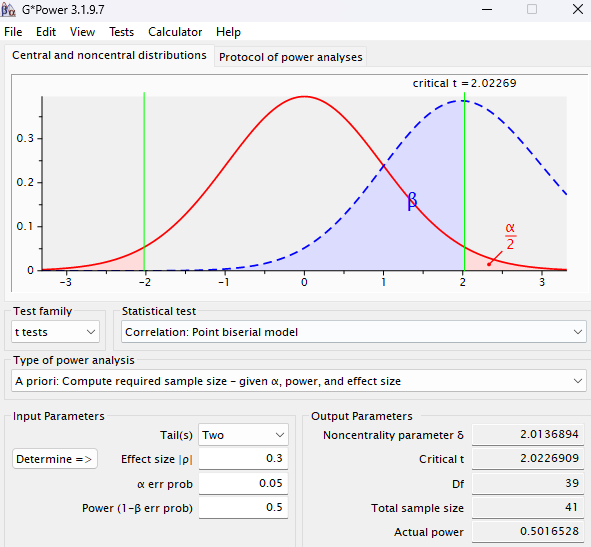
\includegraphics[width=0.8\textwidth]{pics/replilcatte power0.5.png}
			\end{figure}
			
			\column{.6\textwidth}
			\begin{figure}[H]
				\centering
				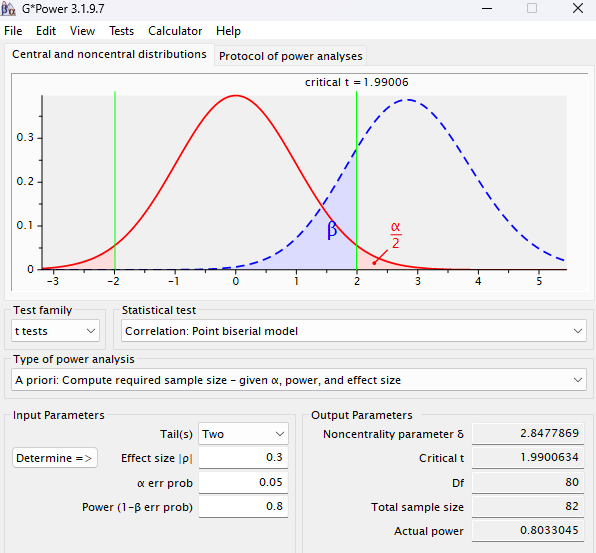
\includegraphics[width=0.8\textwidth]{pics/replilcatte power0.8.png}
			\end{figure}
		\end{columns}	
		
	\end{frame}
	
	\begin{frame}{Hints that sample size should be over 80}
		\begin{figure}[H]
			\centering
			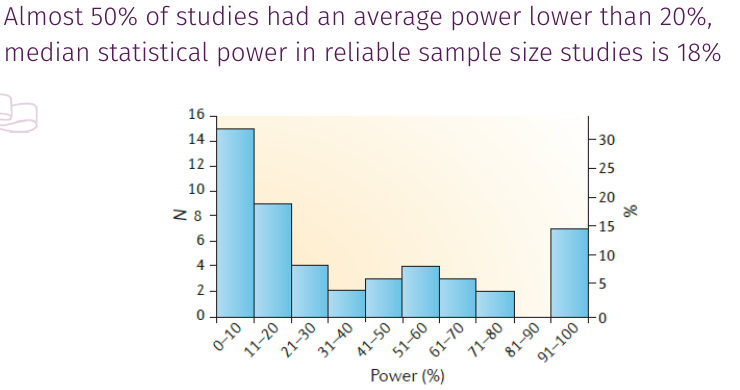
\includegraphics[width=0.8\textwidth]{pics/sample size 80.png}
		\end{figure}
		
		These seven meta-analyses were all broadly neurological in focus and were based on relatively small contributing studies — four out of the seven meta-analyses did not include any study with over 80 participants.
	\end{frame}
	
	\begin{frame}
		\begin{center}
			\textbf{Thank you for your attention!}
		\end{center}
		
		\begin{figure}[H]
			\centering
			
\includegraphics[width=1\textwidth]{pics/hatch.png}
		\end{figure}
	\end{frame}
	
%    \section{References}

    \begin{frame}{References}
%		\begingroup
%		\tiny 
%		\AtNextBibliography{\tiny}
		\printbibliography[heading=none]
%		\endgroup
    \end{frame}
\end{document}